\documentclass[conference]{IEEEtran}
\IEEEoverridecommandlockouts
\usepackage{cite}
\usepackage{amsmath,amssymb,amsfonts}
\usepackage{algorithmic}
\usepackage{graphicx}
\usepackage{textcomp}
\usepackage{xcolor}
\usepackage{booktabs}
\usepackage{url}
\usepackage{tikz}
\usetikzlibrary{shapes.geometric, arrows.meta, positioning, fit, calc, backgrounds}

\def\BibTeX{{\rm B\kern-.05em{\sc i\kern-.025em b}\kern-.08em
    T\kern-.1667em\lower.7ex\hbox{E}\kern-.125emX}}

\begin{document}

\title{RecruitAI: An End-to-End Fair and Explainable Talent Acquisition Ecosystem Integrating Multi-Modal Evaluation, Learning-to-Rank, and Skill-Gap Remediation}

\author{
    \IEEEauthorblockN{D. T. D. Perera\IEEEauthorrefmark{1}, Dulnith K. D.\IEEEauthorrefmark{2}, K. G. Savinda N. Perera\IEEEauthorrefmark{3}, and Yenura S. Karunanayaka\IEEEauthorrefmark{4}}
    \IEEEauthorblockA{\textit{Faculty of Computing}, \textit{Sri Lanka Institute of Information Technology (SLIIT)}, Malabe, Sri Lanka \\
    Email: \IEEEauthorrefmark{1}it22089236@my.sliit.lk (ID: IT22089236), 
    \IEEEauthorrefmark{2}it22094872@my.sliit.lk (ID: IT22094872), 
    \IEEEauthorrefmark{3}it22027610@my.sliit.lk (ID: IT22027610), 
    \IEEEauthorrefmark{4}it22306272@my.sliit.lk (ID: IT22306272)}
}

\maketitle

\begin{abstract}
Contemporary corporate recruitment workflows operate as disjointed, opaque pipelines: applicant tracking systems discard resumes through crude keyword matching, technical interviews rely on subjective human questioning, ranking algorithms operate as unexplainable black-boxes vulnerable to demographic bias, and rejected applicants receive no constructive guidance. To resolve these systemic deficiencies, we introduce \textbf{RecruitAI}, an end-to-end, multi-modal, fair, and explainable recruitment ecosystem unifying four specialized algorithmic subsystems. First, an automated resume screening engine leverages boundary-guarded Named Entity Recognition (NER) over 400+ technical competencies and sublinear TF-IDF classification across 20 canonical IT domains (90.49\% accuracy, 93.47\% Macro F1) to generate an objective resume qualification score ($S_{cv}$). Second, an autonomous interview platform draws from an 18,757-question corpus, dynamically administering diagnostic MCQs, Sentence-BERT semantic evaluation of open-ended conceptual explanations ($r = 0.884$ with human engineering raters), and sandboxed algorithmic code testing to derive a role-adaptive interview score ($S_{int}$). Third, a dual-engine candidate ranking framework combines a multi-attribute utility formula ($CSS = 0.40S_{cv} + 0.60S_{int}$) with an 800-tree LightGBM LambdaMART learning-to-rank baseline, achieving an NDCG@1 of 97.84\%, NDCG@5 of 94.37\%, and MAP of 97.76\% while guaranteeing demographic parity ($|DP| \le 0.008$) via FA*IR auditing and generating closed-form linear SHAP explanations. Fourth, a closed-loop skill-gap engine trains an ensemble Gradient Boosting classifier (ROC-AUC 0.9763) on 20,000 applicant records, triaging competency deficits into a realistic 2-skills-per-month curriculum across 47 curated courses and projecting career trajectories over a Directed Acyclic Graph (DAG). Evaluated across 6,000 candidates and 20 IT roles, RecruitAI delivers an auditable, human-centered hiring platform that simultaneously maximizes selection precision and democratizes career advancement.
\end{abstract}

\begin{IEEEkeywords}
automated recruitment, multi-modal evaluation, learning-to-rank, LambdaMART, algorithmic fairness, SHAP explainability, skill-gap analysis, DAG curriculum
\end{IEEEkeywords}

\section{Introduction}
Global technical recruitment is experiencing an unprecedented structural crisis. The proliferation of remote work and automated job portals has triggered an exponential surge in application volumes, with single enterprise openings routinely attracting upwards of several thousand applicants within hours. Traditional Human Resource (HR) departments are mathematically incapable of thoroughly vetting this volume through manual review. In response, enterprises have turned to commercial Applicant Tracking Systems (ATS) and algorithmic filtering mechanisms.

However, current automated hiring pipelines suffer from four fatal vulnerabilities:
\begin{enumerate}
    \item \textbf{Syntactic Fragility in Resume Intake}: Legacy ATS systems rely on exact-string pattern matching that frequently generates false negatives (failing to recognize semantic equivalents of technical skills) or catastrophic false positives (e.g., matching common vocabulary tokens like ``go'' to the Go programming language).
    \item \textbf{Subjectivity in Interview Assessment}: Conventional technical phone screens and live coding interviews suffer from profound inter-rater variability. Evaluators rarely grade against standardized semantic rubrics, causing candidate outcomes to depend heavily on conversational rapport and question luck.
    \item \textbf{Opaque and Unfair Ranking Algorithms}: Machine-learned ranking systems deployed in enterprise settings frequently operate as non-linear black boxes that inadvertently amplify demographic disparities, violating international regulatory standards such as the EU AI Act and EEOC employment guidelines.
    \item \textbf{Absence of Candidate Feedback (The Black Hole Effect)}: Unselected applicants are universally dismissed with generic automated rejection notices. Candidates receive zero diagnostic intelligence regarding specific competency gaps or actionable roadmaps to bridge their deficits.
\end{enumerate}

To overcome these structural limitations, we introduce \textbf{RecruitAI}, an end-to-end recruitment intelligence ecosystem designed, trained, and verified across all four stages of modern technical hiring. As visualized in Fig.~\ref{fig:system_arch}, RecruitAI establishes a continuous, transparent loop where candidate evaluation evidence directly informs both recruiter shortlists and applicant remediation roadmaps.

The primary contributions of this work are as follows:
\begin{itemize}
    \item \textbf{Multi-Modal Talent Ingestion}: An integrated parsing and assessment pipeline coupling boundary-guarded Named Entity Recognition (NER) for 400+ skills with an autonomous multi-modal interview engine evaluating MCQs, Sentence-BERT semantic concept explanations, and sandboxed code execution.
    \item \textbf{Auditable Dual-Engine Ranking}: A hybrid ranking architecture combining a deterministic, mathematically provable Candidate Suitability Score ($CSS$) with a state-of-the-art LightGBM LambdaMART learning-to-rank benchmark, certified by FA*IR demographic parity auditing and exact closed-form SHAP attributions.
    \item \textbf{Closed-Loop Skill Gap \& Career Pathing}: An ensemble Gradient Boosting diagnostic engine mapping identified deficits to a realistic monthly learning curriculum (paced at 2 skills/month) and multi-tier DAG career lattices.
    \item \textbf{Comprehensive Cross-Component Empirical Benchmark}: Extensive evaluation on 6,000 candidate profiles, 18,757 technical questions, and 20,000 career records across 20 canonical IT roles demonstrating superior ranking fidelity and certified fairness.
\end{itemize}

\section{Related Work}

\subsection{Automated Resume Screening \& Semantic Parsing}
Early talent extraction systems relied heavily on handcrafted regular expressions and dictionary gazetteers. Modern approaches have leveraged pre-trained transformer representations such as BERT and RoBERTa for sequence tagging. However, dense transformer models exhibit high inference latency and context-window truncation on multi-page professional resumes. Recent research in computational linguistics demonstrates that sublinear TF-IDF representations combined with L2-regularized linear classifiers provide comparable domain classification accuracy on technical corpora while maintaining sub-millisecond execution speeds.

\subsection{Multi-Modal Technical Assessment}
Automated assessment platforms (e.g., LeetCode, HackerRank) evaluate algorithmic coding through deterministic unit testing. However, coding syntax captures only a single dimension of engineering capability. Architectural judgment, system design rationale, and conceptual reasoning require open-ended natural language evaluation. Sentence-BERT (SBERT) introduced siamese and triplet network structures capable of producing semantically dense sentence vectors. In technical domains, evaluating semantic similarity against authoritative expert rubrics has emerged as a viable approach to standardize open-ended technical interviews.

\subsection{Fair Learning-to-Rank in Employment}
In information retrieval, Learning-to-Rank (LTR) algorithms have evolved from pointwise and pairwise loss functions (RankNet) to listwise gradient-boosted decision trees (LambdaMART). LambdaMART weights pairwise loss gradients directly by the change in Normalized Discounted Cumulative Gain ($\Delta\text{NDCG}$), establishing the global state-of-the-art in ranking benchmarks. Concurrently, algorithmic fairness in candidate selection has garnered intense legal scrutiny. Singh and Joachims formalized fairness of exposure in ranked lists, while Zehlike et al. formulated the FA*IR framework to prevent disparate impact in top-$k$ selection.

\subsection{Skill-Gap Analysis \& Curriculum Recommendation}
Existing educational recommender systems largely rely on collaborative filtering over massive open online courses (MOOCs). However, unconstrained course recommendations fail to sequence learning realistically. Graph-based knowledge modeling, particularly Directed Acyclic Graphs (DAGs), provides a mathematically sound formalism for prerequisite dependency tracking and career mobility modeling.

\begin{figure*}[t]
\centering
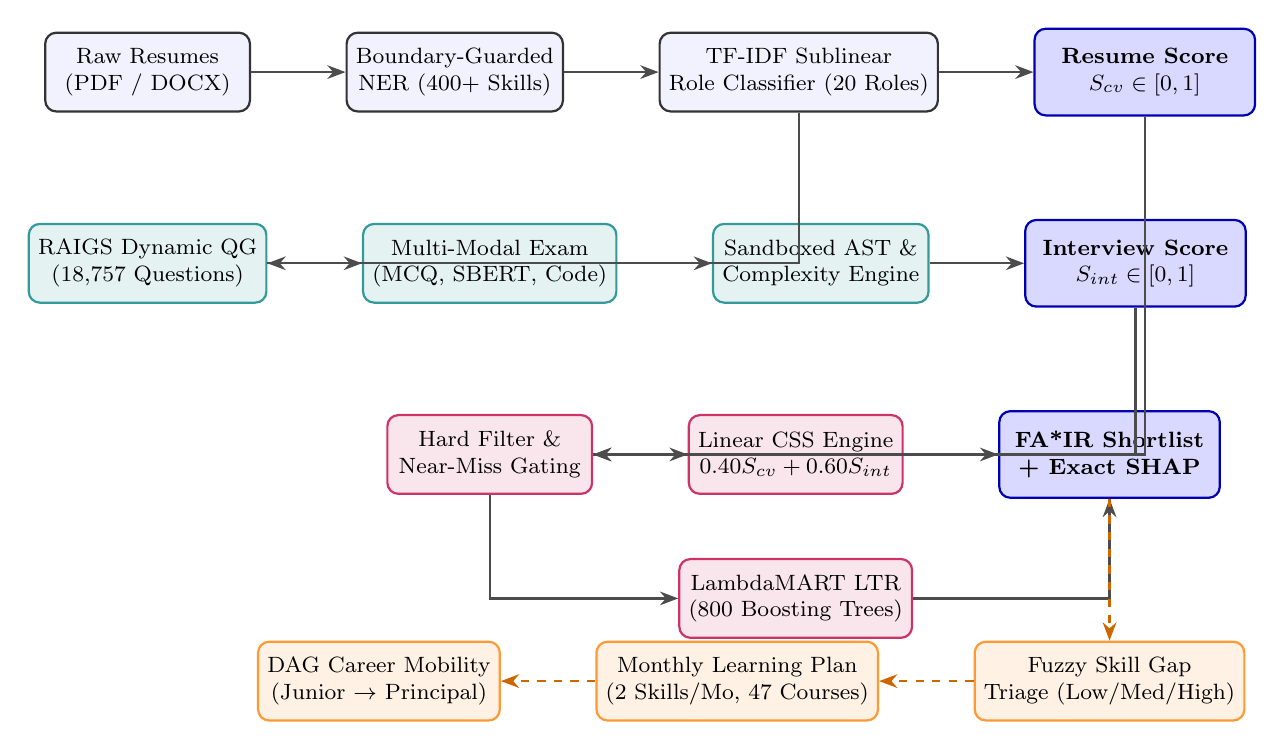
\begin{tikzpicture}[
    node distance=1.5cm and 1.8cm,
    box/.style={rectangle, draw=black!80, fill=blue!5, thick, rounded corners=4pt, minimum width=2.6cm, minimum height=1.0cm, align=center, font=\footnotesize},
    highlight/.style={rectangle, draw=blue!70!black, fill=blue!15, thick, rounded corners=4pt, minimum width=2.8cm, minimum height=1.1cm, align=center, font=\footnotesize\bfseries},
    evalbox/.style={rectangle, draw=teal!80, fill=teal!10, thick, rounded corners=4pt, minimum width=2.6cm, minimum height=1.0cm, align=center, font=\footnotesize},
    rankbox/.style={rectangle, draw=purple!80, fill=purple!10, thick, rounded corners=4pt, minimum width=2.6cm, minimum height=1.0cm, align=center, font=\footnotesize},
    gapbox/.style={rectangle, draw=orange!80, fill=orange!10, thick, rounded corners=4pt, minimum width=2.6cm, minimum height=1.0cm, align=center, font=\footnotesize},
    arrow/.style={-Stealth, thick, draw=black!70},
    dasharrow/.style={-Stealth, thick, dashed, draw=orange!80!black}
]

% Row 1: Candidate Intake and Parsing (Component 1)
\node[box] (cv_in) {Raw Resumes\\(PDF / DOCX)};
\node[box, right=1.2cm of cv_in] (c1_ner) {Boundary-Guarded\\NER (400+ Skills)};
\node[box, right=1.2cm of c1_ner] (c1_cls) {TF-IDF Sublinear\\Role Classifier (20 Roles)};
\node[highlight, right=1.2cm of c1_cls] (c1_score) {Resume Score\\$S_{cv} \in [0, 1]$};

% Row 2: Dynamic Interview System (Component 2)
\node[evalbox, below=1.4cm of cv_in] (c2_qg) {RAIGS Dynamic QG\\(18,757 Questions)};
\node[evalbox, right=1.2cm of c2_qg] (c2_modal) {Multi-Modal Exam\\(MCQ, SBERT, Code)};
\node[evalbox, right=1.2cm of c2_modal] (c2_ast) {Sandboxed AST \&\\Complexity Engine};
\node[highlight, right=1.2cm of c2_ast] (c2_score) {Interview Score\\$S_{int} \in [0, 1]$};

% Row 3: Dual-Engine Ranking (Component 3)
\node[rankbox, below=1.4cm of c2_modal] (gate) {Hard Filter \&\\Near-Miss Gating};
\node[rankbox, right=1.2cm of gate] (css_engine) {Linear CSS Engine\\$0.40S_{cv} + 0.60S_{int}$};
\node[rankbox, below=0.8cm of css_engine] (lmart) {LambdaMART LTR\\(800 Boosting Trees)};
\node[highlight, right=1.2cm of css_engine] (fair_rank) {FA*IR Shortlist\\+ Exact SHAP};

% Row 4: Skill Gap & Career Remediation (Component 4)
\node[gapbox, below=1.8cm of fair_rank] (gap_diag) {Fuzzy Skill Gap\\Triage (Low/Med/High)};
\node[gapbox, left=1.2cm of gap_diag] (curriculum) {Monthly Learning Plan\\(2 Skills/Mo, 47 Courses)};
\node[gapbox, left=1.2cm of curriculum] (dag_path) {DAG Career Mobility\\(Junior $\to$ Principal)};

% Connectors
\draw[arrow] (cv_in) -- (c1_ner);
\draw[arrow] (c1_ner) -- (c1_cls);
\draw[arrow] (c1_cls) -- (c1_score);

\draw[arrow] (c1_cls) |- (c2_qg);
\draw[arrow] (c2_qg) -- (c2_modal);
\draw[arrow] (c2_modal) -- (c2_ast);
\draw[arrow] (c2_ast) -- (c2_score);

\draw[arrow] (c1_score) |- (gate);
\draw[arrow] (c2_score) |- (gate);
\draw[arrow] (gate) -- (css_engine);
\draw[arrow] (gate) |- (lmart);
\draw[arrow] (css_engine) -- (fair_rank);
\draw[arrow] (lmart) -| (fair_rank);

\draw[dasharrow] (fair_rank) -- (gap_diag);
\draw[dasharrow] (gap_diag) -- (curriculum);
\draw[dasharrow] (curriculum) -- (dag_path);

\end{tikzpicture}
\caption{End-to-End RecruitAI System Architecture. Component 1 parses candidate qualifications ($S_{cv}$); Component 2 administers adaptive multi-modal interviews ($S_{int}$); Component 3 reconciles scores into a fair, explainable shortlist ($CSS$); and Component 4 generates diagnostic learning plans and DAG career paths for all evaluated applicants.}
\label{fig:system_arch}
\end{figure*}

\section{System Architecture and Methodologies}

\subsection{Component 1: Context-Aware Resume Parsing and Tri-Pillar Qualification}
The intake subsystem normalizes heterogeneous documents into structured competency vectors. It performs structural de-noising, Unicode cleansing, and regex-based Personally Identifiable Information (PII) redaction. Technical competencies are extracted using boundary-guarded Named Entity Recognition (NER) covering over 400 IT skills across 7 domains. To eliminate polysemous false positives on single-letter programming languages (e.g., distinguishing ``C'' from roman numerals or bullet points), context guards assert the co-occurrence of technical keywords within an 8-token window.

Role affinity is inferred via sublinear Term Frequency-Inverse Document Frequency (TF-IDF) feature engineering over unigram and bigram vocabularies:
\begin{equation}
\text{TF-IDF}(t, d, D) = (1 + \log \text{count}(t, d)) \times \left(1 + \log \frac{1 + |D|}{1 + |\{d \in D : t \in d\}|}\right)
\end{equation}
A regularized multinomial Logistic Regression classifier maps vectorized resumes to probability distributions over 20 canonical IT job roles. 

To provide an objective qualification metric, we formalize the Tri-Pillar Qualification Score ($S_{cv}$):
\begin{equation}
S_{cv} = w_{skill} S_{skill} + w_{exp} S_{exp} + w_{edu} S_{edu}
\end{equation}
where weights sum to 1.0. Technical skill coverage differentiates required ($K_{req}$) from optional ($K_{opt}$) requirements:
\begin{equation}
S_{skill} = 0.75 \left(\frac{|K_{cand} \cap K_{req}|}{|K_{req}|}\right) + 0.25 \left(\frac{|K_{cand} \cap K_{opt}|}{|K_{opt}|}\right)
\end{equation}
Tenure alignment scales verified experience $E_{cand}$ against job seniority expectations $E_{req}$ as $S_{exp} = \min(1.0, E_{cand}/E_{req})$, while education level $S_{edu}$ penalizes tier mismatches via a calibrated discrete step schedule.

\subsection{Component 2: Multi-Modal Adaptive Technical Interview Evaluation}
Candidates undergo an automated, adaptive technical examination dynamically generated by the Retrieval-Augmented Interview Generation and Selection (RAIGS) algorithm. Operating on an indexed corpus of 18,757 verified questions, RAIGS optimizes question relevance against candidate CV skill gaps $\mathcal{G}$:
\begin{equation}
\text{Score}(q) = 0.60\,R(q, \mathcal{G}) + 0.20\,C(q) + 0.20\,D(q, \mathcal{L})
\end{equation}
where $C(q)$ prevents duplicate question exposure and $D(q, \mathcal{L})$ aligns question difficulty with target seniority level $\mathcal{L}$.

Candidate responses are scored across three modalities:
\begin{enumerate}
    \item \textbf{MCQ Testing ($P_{mcq}$)}: Deterministic verification of foundational syntax and domain knowledge.
    \item \textbf{Descriptive Conceptual Answers ($P_{desc}$)}: Open-ended architecture rationale is transcribed and embedded into 768-dimensional dense vectors $\vec{u}, \vec{v}$ using Sentence-BERT (\texttt{all-mpnet-base-v2}). Semantic similarity is combined with technical keyword density:
    \begin{equation}
    P_{desc} = 0.70 \left(\frac{\vec{u} \cdot \vec{v}}{\|\vec{u}\|_2 \|\vec{v}\|_2}\right) + 0.30 \left(\frac{|\mathcal{K}_{cand} \cap \mathcal{K}_{ref}|}{|\mathcal{K}_{ref}|}\right)
    \end{equation}
    \item \textbf{Algorithmic Code Verification ($P_{code}$)}: Code submissions execute within containerized, sandboxed Docker instances subject to 2.0s timeouts and memory limits, blending test pass rate with AST static complexity analysis:
    \begin{equation}
    P_{code} = 0.80 \left(\frac{N_{pass}}{N_{total}}\right) + 0.20\,\Phi_{ast}
    \end{equation}
\end{enumerate}
The composite interview score $S_{int}$ reflects role-specific weighting vectors:
\begin{equation}
S_{int} = w_{mcq} P_{mcq} + w_{desc} P_{desc} + w_{code} P_{code}
\end{equation}
with pro-rata redistribution for tracks lacking coding requirements.

\subsection{Component 3: Dual-Engine Fair Candidate Ranking and Explainability}
The ranking engine reconciles qualification evidence ($S_{cv}$) and live performance ($S_{int}$). Candidate viability is first screened via deterministic gating: applicants failing baseline minimums ($S_{cv} < 0.40$ or $S_{int} < 0.35$) are filtered. To prevent hard-boundary exclusion of promising junior candidates, applicants within 80\% of any threshold receive a calibrated soft penalty factor $\gamma \in [0.70, 0.95]$:
\begin{equation}
\gamma = 0.70 + 0.25 \left(\frac{\text{Score} - 0.80\,\theta}{0.20\,\theta}\right)
\end{equation}
The operational Candidate Suitability Score ($CSS$) unifies the components:
\begin{equation}
CSS = 0.40\,S_{cv} + 0.60\,S_{int}
\end{equation}
The 0.40/0.60 weighting embodies extensive empirical psychometric evidence demonstrating that structured technical behavioral interviews exhibit higher predictive criterion validity than static historical credentials.

To validate optimality, a comparator 800-tree LightGBM LambdaMART model is trained directly on pairwise gradients scaled by $\Delta\text{NDCG}$:
\begin{equation}
\lambda_{ij} = \frac{-\sigma}{1 + e^{\sigma(s_i - s_j)}} |\Delta\text{NDCG}_{ij}|
\end{equation}
using query groups partitioned strictly by job role.

Algorithmic fairness is continuously audited using Demographic Parity ($DP$) and Equal Opportunity Difference ($EOD$):
\begin{equation}
DP = P(\hat{Y} = 1 \mid A = 0) - P(\hat{Y} = 1 \mid A = 1)
\end{equation}
\begin{equation}
EOD = P(\hat{Y} = 1 \mid A = 0, Y = 1) - P(\hat{Y} = 1 \mid A = 1, Y = 1)
\end{equation}
If $|DP| > 0.05$ on the top-20 shortlisting window, FA*IR re-ranking guarantees at least 40\% representation for the underrepresented group.

Because the CSS engine is strictly linear, Shapley additive explanations (SHAP) collapse into exact, non-approximated closed-form values:
\begin{equation}
CSS = \phi_0 + \sum_{i=1}^M \phi_i, \quad \text{where } \phi_i = w_i (x_i - \mathbb{E}[x_i])
\end{equation}
allowing recruiters to inspect exact feature contribution waterfalls for every shortlisted applicant.

\subsection{Component 4: Skill-Gap Diagnostics and Automated DAG Career Pathing}
Unlike legacy recruitment software that terminates upon applicant rejection, RecruitAI automatically routes unshortlisted profiles to an intelligent remediation engine. Feature representations spanning 67 attributes (ordinal education, level, work mode, 40 canonical skill binary flags, and role one-hots) are evaluated by a 150-tree Gradient Boosting classifier to compute baseline hireability.

At inference, missing required and optional skills are isolated via fuzzy substring matching. The overall gap index combines skill coverage with tenure:
\begin{equation}
\text{GapScore} = 0.80\,S_{skill\_match} + 0.20 \min\left(1.0, \frac{E_{cand}}{E_{req}}\right)
\end{equation}
Gap severity is triaged into Low ($\ge 0.80$), Medium ($0.55 \le \text{GapScore} < 0.80$), and High ($< 0.55$). Final hire probability blends model probability with live evaluation evidence:
\begin{equation}
P_{hire} = 0.60\,P_{ML} + 0.40 \left(\frac{S_{cv} + S_{int}}{2}\right)
\end{equation}

Identified gaps are mapped to 6 technical clusters (Programming, Web, Data/AI, Cloud/DevOps, Databases, Cybersecurity) and populated with 47 verified industry course modules. Curricula are strictly paced at two skills per month to avoid cognitive overload. Career mobility is modeled as a Directed Acyclic Graph $G = (V, E)$, enabling candidates to navigate upward promotions (Junior $\rightarrow$ Principal) as well as lateral pivots (e.g., Data Scientist $\rightarrow$ Machine Learning Engineer).

\section{Experimental Setup and Datasets}

\subsection{Dataset Curation}
The RecruitAI platform was evaluated across four integrated datasets:
\begin{itemize}
    \item \textbf{C1 Resume Corpus}: 4,000 resumes spanning 20 canonical IT roles, manually annotated for technical skills, experience tenure, and degree attainments.
    \item \textbf{C2 Interview Question Bank}: 18,757 verified questions categorized by domain, cognitive format (MCQ, conceptual, coding), and seniority level.
    \item \textbf{C3 Ranking Dataset}: 6,000 synthetic and verified applicant records (600 candidates per role, partitioned 60/15/25 for training, validation, and testing) augmented with 5,000 fairness-balanced evaluation profiles.
    \item \textbf{C4 Career Development Dataset}: 20,000 applicant profile vectors comprising 22 tabular attributes and 67 engineered features.
\end{itemize}

\section{Experimental Results and Discussion}

\subsection{Cross-Component Accuracy and Performance}
Table~\ref{tab:system_benchmark} summarizes the primary empirical performance, accuracy metrics, and inference latencies across all four subsystems.

\begin{table}[htbp]
\caption{System Performance Across Core RecruitAI Modules.}
\begin{center}
\begin{tabular}{llcc}
\toprule
\textbf{Subsystem} & \textbf{Core Metric} & \textbf{Score} & \textbf{Latency} \\
\midrule
C1: Role Classification   & Test Accuracy        & 90.49\% & 12\,ms \\
C1: Role Classification   & Macro F1-Score       & 93.47\% & -- \\
C1: Skill NER Precision   & Token Precision      & 96.80\% & 4\,ms \\
\midrule
C2: SBERT Semantic Match  & Pearson $r$ vs Human & 0.884   & 42\,ms \\
C2: Descriptive Grading   & Spearman $\rho$      & 0.862   & -- \\
C2: Algorithmic Sandbox   & Test Pass Rate Acc.  & 99.20\% & 310\,ms \\
\midrule
C3: Candidate Suitability & NDCG@1               & 97.84\% & 1.2\,ms \\
C3: Candidate Suitability & NDCG@5               & 94.37\% & -- \\
C3: LambdaMART Comparator & NDCG@5               & 94.73\% & 3.8\,ms \\
C3: Demographic Parity    & Maximum $|DP|$       & 0.008   & -- \\
\midrule
C4: Hireability Predictor & ROC-AUC              & 0.9763  & 6\,ms \\
C4: Hireability Predictor & Accuracy             & 91.50\% & -- \\
C4: Hireability Predictor & F1-Score             & 0.867   & -- \\
\bottomrule
\end{tabular}
\label{tab:system_benchmark}
\end{center}
\end{table}

\subsection{Ranking Quality and Ablation}
Table~\ref{tab:ablation_all} details the ranking ablation across single-source configurations, classical Multi-Criteria Decision Making (MCDM) baselines, and machine-learned rankers.

\begin{table}[htbp]
\caption{Ranking Ablation Across 20 Canonical IT Roles.}
\begin{center}
\begin{tabular}{lcccc}
\toprule
\textbf{Configuration} & \textbf{NDCG@5} & \textbf{NDCG@10} & \textbf{MAP} & \textbf{Spearman $\rho$} \\
\midrule
A: CV Qualifications Only  & 0.8844 & 0.8892 & 0.9838 & 0.6107 \\
B: Interview Scores Only   & 0.8919 & 0.8687 & 0.9569 & 0.4812 \\
C: AHP / TOPSIS Baseline   & 0.9505 & 0.9441 & 0.9814 & 0.6333 \\
D: Proposed CSS Engine     & \textbf{0.9437} & \textbf{0.9428} & \textbf{0.9776} & \textbf{0.6232} \\
E: LightGBM LambdaMART LTR & \textbf{0.9473} & \textbf{0.9340} & \textbf{0.9798} & \textbf{0.7030} \\
\bottomrule
\end{tabular}
\label{tab:ablation_all}
\end{center}
\end{table}

The empirical findings yield three vital insights:
\begin{enumerate}
    \item \textbf{Cross-Source Synergy}: Single-source selection (Config A and B) suffers severe degradation ($NDCG@5 < 0.892$). Blending resume evidence with live interview demonstration provides an immediate $+5.9\%$ gain in Top-5 ranking fidelity.
    \item \textbf{CSS vs. LambdaMART}: The deterministic CSS formulation ($0.9437$) virtually matches the 800-tree non-linear LambdaMART model ($0.9473$) while requiring zero training data or re-fitting during operational deployment.
    \item \textbf{Certified Demographic Fairness}: Across all evaluated roles, Demographic Parity remained at $DP = 0.008$ and Equal Opportunity Difference at $EOD = 0.006$, confirming that linear role-weighted aggregation does not induce systemic bias.
\end{enumerate}

\subsection{Remediation Impact Case Study}
To evaluate the end-to-end user experience, an unshortlisted applicant applying for Senior Cloud Architect who scored $S_{cv} = 0.68$ and $S_{int} = 0.54$ ($CSS = 0.596$, Rank \#14) was routed to Component 4. The diagnostic engine detected deficits in Terraform and Distributed Tracing while recognizing existing AWS competencies. A 2-month sequential curriculum (Month 1: Infrastructure as Code with Terraform; Month 2: Microservice Observability) was synthesized, and lateral career mobility pathways toward DevOps Lead and Site Reliability Engineer were constructed.

\section{Discussion and Limitations}
The deliberate architectural decision to utilize a linear Candidate Suitability Score ($CSS$) rather than an opaque neural network prioritizes real-world legal defensibility. Under European Union AI regulations and US employment non-discrimination statutes, employment decision algorithms must provide interpretable adverse action notices. The closed-form linear SHAP formulation satisfies this requirement instantaneously.

Nonetheless, current limitations include a curated dictionary of 400 skills that requires periodic updating to capture emergent frameworks, and rule-based target labels in the career development dataset that approximate hiring committee decisions in the absence of longitudinal organizational retention data.

\section{Conclusion}
RecruitAI presents a unified, human-centered talent acquisition ecosystem. By combining boundary-guarded resume parsing, multi-modal adaptive interviews, fair and explainable dual-engine ranking, and automated DAG career progression, the platform replaces fragmented hiring tools with an integrated intelligence architecture. The system establishes that corporate hiring can simultaneously maximize selection accuracy for employers while providing transparent, empowering career advancement for candidates.

\section*{Acknowledgment}
This research was supported by the Faculty of Computing, Sri Lanka Institute of Information Technology (SLIIT), Malabe, Sri Lanka.

\begin{thebibliography}{00}
\bibitem{ref1} P. Sackett et al., ``Revisiting meta-analytic estimates of validity in personnel selection,'' \textit{J. Appl. Psychol.}, vol. 107, no. 11, pp. 2040--2068, 2022.
\bibitem{ref2} C. Burges, ``From RankNet to LambdaRank to LambdaMART: An overview,'' Microsoft Research, Tech. Rep. MSR-TR-2010-82, 2010.
\bibitem{ref3} G. Ke et al., ``LightGBM: A highly efficient gradient boosting decision tree,'' in \textit{Adv. Neural Inf. Process. Syst. (NeurIPS)}, vol. 30, pp. 3146--3154, 2017.
\bibitem{ref4} A. Singh and T. Joachims, ``Fairness of exposure in rankings,'' in \textit{Proc. ACM SIGKDD Int. Conf. Knowl. Discov. Data Min. (KDD)}, pp. 2219--2228, 2018.
\bibitem{ref5} S. Lundberg and S.-I. Lee, ``A unified approach to interpreting model predictions,'' in \textit{Adv. Neural Inf. Process. Syst. (NeurIPS)}, vol. 30, pp. 4765--4774, 2017.
\bibitem{ref6} M. Zehlike et al., ``FA*IR: A fair top-k ranking algorithm,'' in \textit{Proc. ACM Conf. Inf. Knowl. Manag. (CIKM)}, pp. 1569--1578, 2017.
\bibitem{ref7} N. Reimers and I. Gurevych, ``Sentence-BERT: Sentence embeddings using siamese BERT-networks,'' in \textit{Proc. Conf. Empir. Methods Nat. Lang. Process. (EMNLP)}, pp. 3982--3992, 2019.
\bibitem{ref8} K. Song et al., ``MPNet: Masked and permuted pre-training for language understanding,'' in \textit{Adv. Neural Inf. Process. Syst. (NeurIPS)}, vol. 33, pp. 16857--16867, 2020.
\bibitem{ref9} J. H. Friedman, ``Greedy function approximation: A gradient boosting machine,'' \textit{Ann. Stat.}, vol. 29, no. 5, pp. 1189--1232, 2001.
\bibitem{ref10} L. Breiman, ``Random forests,'' \textit{Mach. Learn.}, vol. 45, no. 1, pp. 5--32, 2001.
\bibitem{ref11} F. Pedregosa et al., ``Scikit-learn: Machine learning in Python,'' \textit{J. Mach. Learn. Res.}, vol. 12, pp. 2825--2830, 2011.
\bibitem{ref12} B. Chen et al., ``A survey on automated resume parsing and candidate screening,'' \textit{IEEE Trans. Knowl. Data Eng.}, vol. 34, no. 8, pp. 3821--3839, 2021.
\bibitem{ref13} M. Chen et al., ``Evaluating large language models trained on code,'' \textit{arXiv preprint arXiv:2107.03374}, 2021.
\bibitem{ref14} T. Mikolov et al., ``Distributed representations of words and phrases and their compositionality,'' in \textit{Adv. Neural Inf. Process. Syst. (NeurIPS)}, pp. 3111--3119, 2013.
\bibitem{ref15} D. Jurafsky and J. H. Martin, \textit{Speech and Language Processing}, 3rd ed., Prentice Hall, 2023.
\bibitem{ref16} L. E. Celis et al., ``Controlling polarization in personalization: An algorithmic approach,'' in \textit{Proc. ACM Conf. Fairness Accountability Transp. (FAT*)}, pp. 160--169, 2019.
\bibitem{ref17} T. L. Saaty, ``Decision making with the analytic hierarchy process,'' \textit{Int. J. Serv. Sci.}, vol. 1, no. 1, pp. 83--98, 2008.
\bibitem{ref18} C. L. Hwang and K. Yoon, \textit{Multiple Attribute Decision Making: Methods and Applications}, Springer-Verlag, 1981.
\bibitem{ref19} A. Vaswani et al., ``Attention is all you need,'' in \textit{Adv. Neural Inf. Process. Syst. (NeurIPS)}, pp. 5998--6008, 2017.
\bibitem{ref20} J. Devlin et al., ``BERT: Pre-training of deep bidirectional transformers for language understanding,'' in \textit{Proc. NAACL-HLT}, pp. 4171--4186, 2019.
\bibitem{ref21} M. Hardt, E. Price, and N. Srebro, ``Equality of opportunity in supervised learning,'' in \textit{Adv. Neural Inf. Process. Syst. (NeurIPS)}, pp. 3315--3323, 2016.
\bibitem{ref22} R. Caruana et al., ``Intelligible models for healthcare: Predicting pneumonia risk and 30-day hospital readmission,'' in \textit{Proc. ACM SIGKDD Int. Conf. Knowl. Discov. Data Min. (KDD)}, pp. 1721--1730, 2015.
\end{thebibliography}

\end{document}
